\documentclass[12pt, oneside, a4paper]{book}

\renewcommand{\baselinestretch}{1.25}
\setlength{\parskip}{5pt}
\setlength{\parindent}{0pt}

\usepackage{hyphenat}
\usepackage[pdftex]{graphicx}
\usepackage{pslatex}
\usepackage{comment}
\usepackage[scaled=1.0]{helvet}
\usepackage[utf8]{inputenc}
\usepackage{blindtext}
%\usepackage{styles/minted}
\usepackage{subfig}
\usepackage[justification=centering]{caption}
\usepackage{url}
\usepackage{titlesec}
\usepackage[T1]{fontenc}
\usepackage{epstopdf}
\usepackage{microtype}
\usepackage{color}



%\usepackage{pgf-blur}

% chapters style
\definecolor{gray75}{gray}{0.75}
\newcommand{\hsp}{\hspace{20pt}}
\titleformat{\chapter}[hang]{\Huge\bfseries}{\thechapter\hsp\textcolor{gray75}{|}\hsp}{0pt}{\Huge\bfseries}
\titlespacing{\chapter}{0pt}{0pt}{1cm}

\begin{document}
\inputencoding{utf8}

% *************** Front matter ***************
\frontmatter

\begin{titlepage}

\setlength{\textwidth}{15cm}
\addtolength{\hoffset}{-1.7cm}
\addtolength{\voffset}{-1.8cm}

\vbox to 150mm{

{\fontfamily{phv}\selectfont

\makebox[\textwidth][c]{University of West Bohemia}

\vspace{0.5cm}

\makebox[\textwidth][c]{Faculty of Applied Sciences}

\vspace{0.5cm}

\makebox[\textwidth][c]{Department of Computer Science and Engineering}

\vspace{6cm}

\makebox[\textwidth][c]{\LARGE{\textbf{DIPLOMA THESIS}}}

\vspace{13.3cm}

\makebox[\textwidth][c]{Pilsen, 2013 \hspace{6.5cm} Jan Koreň}



\vss
}


}

\end{titlepage}

\begin{titlepage}

\font\uni=cmr17 at 22pt
\font\dip = cmb10 at 28pt
\font\nam = cmr17 at 16pt

\addtolength{\voffset}{-1.8cm}

\vbox to 150mm{



\makebox[\textwidth][c]{\uni University of West Bohemia}

\vspace{0.5cm}

\makebox[\textwidth][c]{\uni Faculty of Applied Sciences}

\vspace{0.5cm}

\makebox[\textwidth][c]{\uni Department of Computer Science and Engineering}

\vspace{3.5cm}

\makebox[\textwidth][c]{\dip Diploma Thesis}

\vspace{2.5cm}

\makebox[\textwidth][c]{\dip Fulltext search in the database }
\makebox[\textwidth][c]{\dip and in texts of social networks}

\vspace{12.5cm}

\makebox[\textwidth][c]{\nam Pilsen, 2013 \hspace{6.5cm} Jan Koreň}



\vss



}

\end{titlepage}

\thispagestyle{empty}


\section*{Declaration}

I hereby declare that this diploma thesis is completely my own work
and that I used only the cited sources. 


\date{Pilsen, Jan Koreň}

\pagebreak{}


\thispagestyle{empty}

\chapter*{Acknowledgements}

I would like to thank to...

\pagebreak{}


\thispagestyle{empty}


\chapter*{Abstract}


This thesis is focused on design and implementation of the full text
search in EEG/ERP Portal. This full text search capability includes
searching text in the EEG/ERP Portal database as well as in related
data from social networks, such as LinkedIn or Facebook. With the
development of the Portal and the increasing amount of processed data,
a proper full text search mechanism for information retrieval is necessary
for improving the user experience by enabling efficient do\-cu\-ment retrieval. 

\pagebreak{}

%\vspace{5mm}\\
{\bf Keywords}:
Lucene, Solr, full text search

\thispagestyle{empty}

\vfill\eject

\tableofcontents

% *************** Main matter ***************
\mainmatter


\chapter{Introduction}

Accessing required information from a large set of data in a quick and user-friendly manner is no longer an unachievable goal. 
Advancements in the field of information retrieval in the last few decades have made its applications 
very common.
Full text search, as one of such applications, has in fact become an essential part of everyday's life in a modern society.

%, such as full text search, so common 
%that they have become in many cases an essential part of many tasks of everyday's life in a modern society. 
This work deals with the topic of full text search over data belonging to the domain of the EEG/ERP Portal, a piece of software which is being developed at the University of West Bohemia in Pilsen. 

The work is organized into two main parts.
The first part, theoretical part, includes chapters \ref{chap:fulltext}-\ref{chap:eegPortal} and covers theoretical knowledge used throughout the thesis. 
Chapter \ref{chap:fulltext} deals with the problematics of full text search, its core concepts are introduced and a comparison between full text search and relational database systems is made.
Specific open-source full text search engines and libraries are listed in Chapter \ref{chap:engines}.
In Chapter \ref{chap:eegPortal}, the EEG/ERP Portal together with its underlying technologies, which are currently used for its development, are presented. 

The practical part of the thesis is dedicated to creation of the full text search functionality and is formed by chapters \ref{chap:analysis}-\ref{chap:testing}.
% builds upon the theoretical background provided in the theoretical part.
Chapter \ref{chap:analysis} includes analysis of the state of the EEG/ERP Portal before any changes were made, and collecting full text search requirements. 
Based on the requirements, a full text search solution is chosen and the overall system architecture is proposed.
Chapter \ref{chapter:indexDesign} is focused on creating a document model for indexed data, and on all necessary configuration related to indexing and searching these data.
Chapter \ref{chap:implementation} is devoted to implementation of the full text search functionality into the EEG/ERP Portal application.
In Chapter \ref{chap:testing}, unit and integration tests that confirm the functionality of the created code are described.

%Chapter 7 comprises discussion about the chosen implementation and
%potential future work based on results of this thesis.

The final chapter, Chapter \ref{chap:conclusion}, contains a summary of the thesis and presentation of results.



\part{Theoretical Part}

Information and efficient access to it form an essential part of life in a modern society. 
Computing and related technologies have changed the ways textual information is stored, searched and retreived. 
The amount of information has grown rapidly in the last few years due to the information explosion caused mainly by the World Wide Web. 
The result is that nowadays, people are exposed to much more information than they used to be. 
Simple categorization of documents made by humans, although doable, is no longer an efficent method of storing data to be searched. 
Except for the fact that this activity is very time-consuming, it can also be automated. 
In order to manage such amount of data and obtain relevant information within a reasonable time period, new powerful techniques operating on vast collections of data were needed.

The problematics of searching relevant information in large data sets has been an objective of a detailed research for more than sixty years. 
The aim of the following parts is to introduce some fundamental concepts
of information retrieval, a discipline including the full text search,
in the context of full text search and compare these concepts with similar principles used in the relational and
NoSQL database worlds.

The latter chapter describes available open-source full-text engines.



\chapter{Full text Search}

The aim of this chapter is to explain basic concepts applied in full
text search, one of the methods dealing with the problem of searching information.

\section{Information retrieval}

Full text search together with database systems can be considered  as a part of a subdiscipline of computer science known
as information retrieval (IR) \cite{Witten:1999:MGC:323905}.
There is a number of available definitions of information retrieval.
According to \cite{IRDataAlgorithms}, information
retrieval (IR) is loosely defined as

	\begin{quote}
		\textsl{``the subfield of computer science
	that deals with the automated storage and retrieval of documents''}
	\end{quote}

This definition as well as the definitions from other sources (e.g. from \cite{Witten:1999:MGC:323905}) sum up the purpose of IR in a very general way.
While the definition above puts no restrictions to the nature of stored documents in the IR system and therefore comprises both full text search and database systems, there exist stricter IR definitions that do not apply to structured data found typically in relational databases. 
Such definition of IR can be found in \cite{Manning:2008:IIR:1394399}:

	\begin{quote}
		\textsl{``Information retrieval (IR) is finding material (usually documents) of an unstructured nature (usually  text) that satisfies an information need from within large collections (usually stored on computers).''}
	\end{quote}

All IR systems - and full text search engines are no exception - are based on the same architecture which is adapted to requirements the specific systems have. In addition, these systems share common IR terminolgy, whose most important terms are explained in this chapter.

\section{Principles of Full Text Search}

% Ostry text

The field of full text search covers a wide range of topics, including efficient algorithms and data structures in order to enable fast and reliable full text search over large amount (in practice gigabytes) of data. 
It is not the aim of this thesis to provide a deeper, more complex insight into this problematics as the final implementation of the full text search feature will be based on an existing full text search engine. 
However, there are several terms and concepts that must be at least briefly explained so that the reader can fully understand the latter text.


\subsection{Full Text Search Engine Architecture}

As can be seen in schema in Figure ~\ref{fig:fulltext_schema}, full text search engines comprise several steps in order to provide a user with search results to a given \textsl{query}. 
\textsl{Query} is in this case a piece of text to be searched, optionally enriched by special operators which serve for refining the query. It is a \textsl{user} of the IR system who comes up with the query, expecting that the system will fulfill his \textsl{information need} by returning relevant search results.

Search engines need source data to actually perform searching. The basic informational unit which is processed by the search engine and returned to the user in case of match with the query is called \textsl{document}. In this context, a document or a collection of documents inserted to the system are representations of real documents, so a series of data transformations must be made first. These steps are for reasons of clarity not depicted in the schema.
  
\begin{figure}[h]
	\centering
		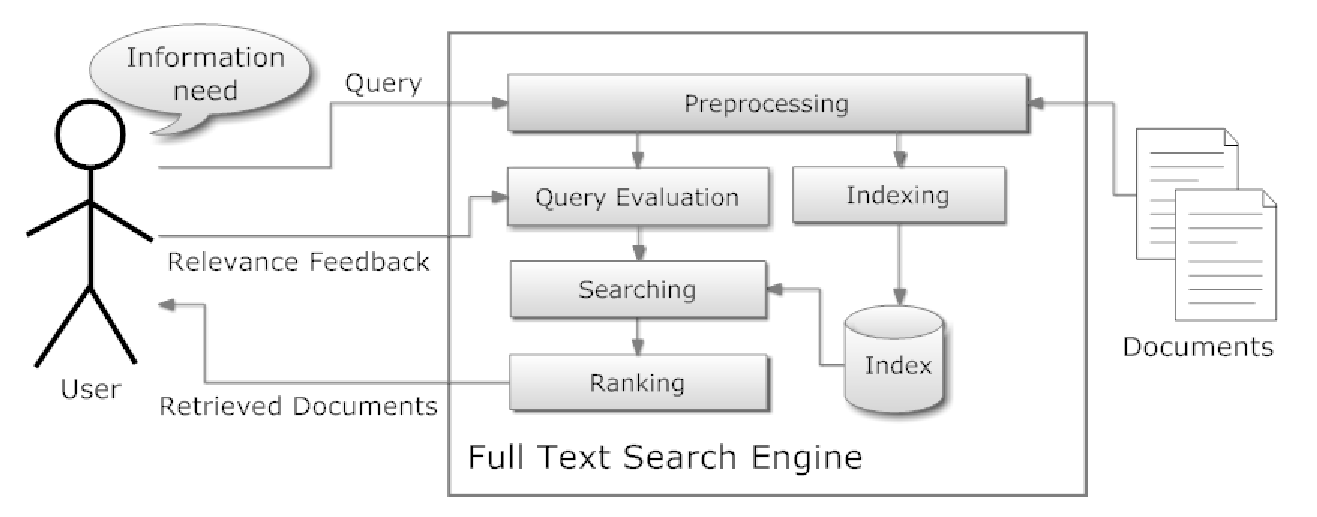
\includegraphics[scale=0.63]{figures/fulltext_schema.eps}
	\caption{IR Architecture Schema. Adapted from \cite{IR:ImplemEvalSearchEng}.}
	\label{fig:fulltext_schema}
\end{figure}

TODO vysvetlit schema, pojmy nize - in progress...

\subsubsection{Preprocessing phase}

Both input query and documents usually undergo several preprocessing steps. These steps, sometimes reffered to as \textsl{filters},   
treat the input text as a stream. 

Tokenization = token stream -> tokens; token normalization -> lowercasing letters, removal of accents, diacritics and so on

separate the text into basic textual units called \textsl{tokens}, in some sources also reffered to as \textsl{words}. These tokens are then operated on. The operations can involve. The result of these operations is a set of terms which are kept in a lexicon of the IR system. 

\subsubsection{Indexing phase}

\subsubsection*{Index}

Index is defined by Frakes \cite{IRDataAlgorithms} the following way: 
	\begin{quote}
	\textsl{``A collection of terms with pointers to places where information about them can be found.''} 	
	\end{quote}
Based on information found in \cite{ManningRaghavanSchuetze08, IRDataAlgorithms, Witten:1999:MGC:323905}, there are three main indexing methods – inverted file, signature file and bitmaps. Based on the comparisons made \cite{Witten:1999:MGC:323905} and in \cite{Zobel:1996:GPC:234889.234891}, using inverted files should be the prefered way due to their faster speed and lower index size required. The remaining two alternatives are recommended to be used only in certain circumstances which are very rare in practice. 

\subsubsection*{Inverted File}

This data structure can be thought of as the well-known index at the end of a book. If we sticked to the IR terminology and characterize it more precisely, we might come up with a more precise characteristics, such as the one found in \cite{Witten:1999:MGC:323905}:

\begin{quote}
		\textsl{``An inverted file contains, for each term in the lexicon, an inverted list that stores a list of pointers to all occurrences of that term in the main text, where each pointer is, in effect, the number of a document in which that term appears.''}
	\end{quote}
	
	To visualize the basic idea of the invered file, Figure  represents a situation of an indexed sentence.
	Obrazek!!!
	
\subsubsection{Query evaluation}

\subsubsection{Searching phase}


\subsubsection*{Boolean query}

\subsubsection*{Ranked query}


\subsubsection{Ranking phase}	


\subsubsection*{Query, Term, Document Operations}

\subsubsection*{Relevance Evaluation}

\subsubsection*{Filters}


% Poznamky

%An IR system matches user queries - formal statements of information
%needs - to documents stored in a database. {[}IRDSA,Frakes{]}
%
%An IR system must support certain basic operations. There must be
%a way to enter documents to a database, change the documents and delete
%them.The must be also some way to search for documents, and present
%them to a user.
%
%and to overcome the informational overload
%
%Though it is possible to keep the index structure in main memory,
%in practice IR databases are usually stored on disk because of their
%size.
%
%Inverted file - a kind of indexed file, the most common solution in
%commercial systems {[}IRDSA,Frakes{]}
%
%The basic item stored in the index 
%
%Todo Lucene in Action and other sources
%
%identify index terms
%
%how to decide if a document matches a query
%
%precision = number of relevant documents retreived divided by the
%total number of documents retreived
%
%recall = number of relevant documents retreived divided by the total
%number of relevant documents
%
%ideally, both parameters should equal to one. This would mean that
%the system returns all relevant documents without introducing any
%irrelevant documents in the results set - impossible to acheive in
%practice.
%
%Improving recall -> precision decreases, likewise improving precision
%at the expense of recall
%
%Furthermore - tradeoff between retreival effectiveness and computing
%cost (key word matching < statistical ranking <\ natural-language
%processing)
%
%Statistical model
%
%Here a document is conceptually represented by a vector of keywords
%extracted from the document, with associated weights representing
%the importance of the keywords in the document and within the whole
%document collection.
%
%Query is modelled as a list of keywords with associated weights representing
%the importance of the keywords in the query.
%

\section{Full text vs. DB search}

Relational database systems and their properties ACID - widely used
for structured data, they are a perfect fit for storing structured
data. As long as these conditions are met relational databases are
a recommended solution for our domain.

traditional search engines - e.g. MySQL databaze. Je zde konstrukce
LIKE (LIKE '\%life\%').

If more terms are searched the underlying query grows in complexity.
Multiple JOIN operations must be used to fetch all data from corresponding
tables, also the query must be written the way to ensure finding the
records with terms not necessarily next to each other as well. As
the query gets more complex, it takes more time to get query results.
Furthermore, the query execution slows down due to the fact that the
query needs to match each term individually.

The query result does not contain any information on the relevancy
of searched terms and found results. Relational database systems simply
output the records matching the criteria.

On the contrary, IR systems provide us with additional relevancy information
of searched terms. Document relevancy is one of the key features of
full text search engines because it is desired to display the results
sorted by their relevance (mostly those most relevant ones are displayed
first).

It is worth mentioning that some DBMS posess native full-text support.
MySQL - keyword FULLTEXT INDEX, for searching on a field, on which full text search will be performed. 
These fulltext indexes are supported only by 
MyISAM engine. They are generally faster than LIKE, however, their usage is limited - vendor lock-in,
moreover, this solution is not unified (implementace,syntaxe se mouhou
can differ, decision to switch to another database could mean interactions to the current system to preserve functionality and scalability. It is bound solely to DBMS - they also lack bigger scaling possibilities and have problems in this area. And it is still slower than external search engines.

{[}IRDSandA,Frakes, p.14{]}:

difference - amount of usable structure in their data objects. Document
generally have less usable structure than the table used by relational
DBMS.

IR - retrieval is probabilistic. No certainity that a retreived document
will meet the informaiton need of the user. (typically, some relevant
documents will be missed, whereas some nonrelevant documents wil be
retreived) vs. DB queries consist of attribute-value pairs that either
match or do not match records in the database.

same - their databases are often very large (can be gigabytes)

same - database volatility - means constant changes as documents are
added, changes or deleted.


\section{Benefits of full text search}

When searching over unstructured data and large data sets, full text
search should be favored to querying relational databases.
\begin{itemize}
\item faster than traditional database search - benefits from word index,
ktery se prochazi pri hledani (jsou pouzity to look up records),
vs. DB - provadi se full table scan
\item found records can be sorted by their relevance. This is called ranking.
\item good performance also over a DB with millions of records
\item ability to skip common words with no additional information. This
depends on the domain languages (in case of English these words include
e.g. the, an, for), search precision can decrease in some cases. 
\end{itemize}
Fulltext pouzijeme, pokud:
\begin{itemize}
\item if there is a lot of unstructured data that are to be looked up
\item it is necessary to get optimized search results.
\item demand for flexible querying
\end{itemize}

\section{Search Engines}

It is a software that is responsible for two steps:
\begin{itemize}
\item building an index on text
\item answering queries by using the created index
\end{itemize}
Compared to databases, it beats them by scalability, relevance ranking,
integration of different data sources (email, web pages, files, database,
...)


\section{Indexing}

Despite various specifics of available search engines, the indexing proces generally consists of several phases.
\cite{Fox:1991:FFA:903195}


\section{Searching Features}

Todo


\chapter{Available Search Engines}
\label{chap:engines}

% http://www.sigir.org/forum/2012D/p095.pdf?searchterm=lucene

% http://stackoverflow.com/questions/737275/comparison-of-full-text-search-engine-lucene-sphinx-postgresql-mysql

% http://php.vrana.cz/fulltextove-vyhledavani-sphinx.php

% http://beerpla.net/2009/09/03/comparison-between-solr-and-sphinx-search-servers-solr-vs-sphinx-fight/

According to the comparisons of fulltext search engines in \cite{MiddletonBaeza} and \cite{SinghSearchEngines}, there are several reasonable options to choose from. 
Unfortunately, there is not enough comparative benchmarks on performance of search engines. Available comparisons are often not so objective since, for example, only the default settings of search engines are used in the tests or just one use case is applied
(as in \cite{SinghSearchEngines}). 
This may lead to false conclusions obtained from these benchmarks because search engines' capabilities might not have been fully demonstrated and tested. 
It is also worth mentioning that some comparisons were made a few years ago and are likely to be out-dated since these technologies evolve quite quickly.
All these experiments showed, however, that database fulltext search possibilities are way too slow \cite{BenchmarkLuceneRelDB,BenchmarkMysqlLuceneSphinx}.

In the following paragraphs the reader can grasp a basic overview on several full text search engines which are considered to be fairly
performant and usable for common full text search scenarios.


\section{Indri}

Indri \cite{IndriHome} is an academic C++ based text search engine
developed at the University of Massachusetts and is a part of the
Lemur Project. The engine is interesting because of its implementation
as it combines inference networks with language modeling. Its API
is accessible also from other languages such as Java or C\#. Great
support of scaling and support of true multithreaded operation, enabling
concurrent adding, querying and deleting documents belong to its main
features. In the technical paper \cite{ComparisonLuceneIndri}
it was shown that Indri is very performant and in comparison with
Lucene it achieves even better results in terms of retrieval effectiveness
for short queries, index size and performance.


\section{Lucene}

Lucene \cite{LuceneHome} is an open source Java-based search library. 
It can enrich applications by its ability to index data and search over them. 
These two main items form what is commonly reffered to as Lucene core. 
Apart from the core, its latest version comprises useful features related to full text search problems (e.g. result highlighting). 
Lucene is highly modularized and its API enables a user to extend its functionality relatively easily \cite{McCandless:2010:LAS:1893016}. 

It stores its index as files on disk. When the search is made, segments of indexes are copied to memory, thus its memory consumption is high and mostly stable.

According to \cite{MiddletonBaeza,ComparisonLuceneIndri}, it belongs to the fastest engines and its performance shines especially
when querying one- or two-word phrases. 
Its small size of index it creates is also a plus when the lack of memory could be an issue.
Thanks to its portability and its active development and active and numerous community, it has become the leading open source search engine used in many successful projects \cite{LuceneWhoUses}.

According to its official documentation \cite{LuceneScoring}, 
\textit{``Lucene scoring uses a combination of the Vector Space Model (VSM) of Information Retrieval and the Boolean model''}.
The Boolean model is used to filter the documents that are then scored.

The current version of Lucene, Lucene 4.0, \textit{,,represents a significant milestone in the development of Lucene due to a number of new features and efficiency improvements as compared to previous versions of Lucene.``} \cite{ApacheLucene4}


\section{Sphinx}

Sphinx \cite{SphinxHome} is an open source search server distributed under GPL license. 
It consists of an indexing tool, which is also referred to as indexer, and a searching daemon. 
Sphinx is written in C++ and is especially designed for indexing database systems (it integrates well with MySQL).
The reason behind its connection with MySQL RDBMS is to enable efficient full-text search on a large amount of database data \cite{aksyonoff2011introduction}.
It allows a user to issue queries with SQL-like syntax for indexing the database content and searching in the index.
Besides database indexing, it also supports an XML format for arbitrary data. 
Considering results from all found benchmarks involving Sphinx \cite{IndriHome,MiddletonBaeza,BenchmarkLuceneSphinxNewer,BenchmarkMysqlLuceneSphinx}, its indexing speed is quick and its search speed belongs to the fastest ones. 
It offers API bindings for several platforms/languages, including Java. 
Among its strengths we can name quick installation and deployment and a perfect online documentation for an open source project. 
Extensibility is quite an issue if our application requires additional features
\cite{esSphinxLuceneSolXapianWhich}. 

\section{Xapian}

According to information found on its official website \cite{XapianHome}, it is an open-source search library written in C++ based on a probabilistic retrieval model. 
It provides a user with bindings that allow to use it from a couple of other languages, including Java, C\# or Ruby. 
Its index size is generally larger when compared to other search engines, but this extra piece of information contained in the index allows Xapian to delete or update a document in a more correct way. 
It is done by storing a list of elements in each document in the termlist table\cite{XapianIndexSize}. 
The benchmarks in \cite{SinghSearchEngines} from 2009 show that its search performance is said to be equally good as the one of Lucene.

\section{Zettair}

Another search engine that received a very positive rating in \cite{MiddletonBaeza} is Zettair \cite{ZettairHome}. 
The comparison in this paper concludes that Zettair has the fastest indexer, provides fast querying speeds and has also the best retrieval effectiveness on average. 
Zettair is being developed at the Australian university and is written entirely in C. 
One of its main features is the ability to handle large data sets (100 GB and more) due to its scalability to large collections \cite{ZettairHome}.

Among its disadvantages belong its inability to index nothing else than text and html and the fact that the index cannot be built in
parallel using multiple machines. 
There are currently no ports to other languages available, so the full text search, when using Zettair, must be implemented in C.


\section{Lucene-based Search Solutions}
\label{sec:luceneBasedSolutions}

Popularity of Lucene is reflected in the existence of several search solutions which are based on this search library.
Because Lucene itself as a search library provides the core functionality, i.e. indexing and searching documents, its direct integration in applications without any additional enhancements can be cumbersome in the most common use cases.
Unless there are special requirements involving access to low-level APIs of Lucene, opting for the already proved search solutions is recommended \cite{Solr3EnterpriseSS}.

The solutions built on top of Lucene can be divided into \textit{search tools} and \textit{search servers}. 
Search tools extend Lucene in a specific way to cover the problem domain and can be embedded to an application in a form of a library. 
They are usually dependent on other technologies which must be included in the target application. 
A widely used example of such search tool is \textit{Hibernate Search}.
Search servers, on the other hand, are fully independent standalone applications which communicate with the application typically by using the HTTP protocol. The representatives of this category are \textit{Solr} and \textit{ElasticSearch}.


\subsubsection{Hibernate Search}

Hibernate Search \cite{HibernateSearchHome} is an enterprise search tool that forms a bridge between Hibernate and Lucene. 
The aim of Hibernate Search is to enable full text search over persistent domain model by overcoming certain mismatches between the domain model and simple Lucene documents.
In order to make Hibernate Search work, Hibernate or JPA must be used as an object-relational mapping between Java objects and database tables. 
% It leverages the power of Lucene for indexing and searching.
% and of Solr (more about Solr can be found in section 3.6.2), whose of useful features and analyzers can be used. 
It manipulates with persisted Hibernate entities and makes them searchable by adding them in the Lucene index. 
By default, Hibernate Search automatically updates Lucene index after an object is saved or updated by using Hibernate.
In order to achieve indexing of Hibernate entities, created model classes must be enriched of specific Hibernate Search annotations for full text search purposes.
Apart from annotating the entities that should be indexed, no extra configuration is needed. 


\subsubsection{Solr}

Solr \cite{SolrHome} is an open source search server built on top of Lucene which runs within a servlet container such as Jetty or Tomcat.
Because it can be considered as a Lucene extension, most of the Lucene terminology is used for Solr as well. 
Unlike Lucene, document fields have to be defined in the application schema file.

Solr extends Lucene by providing many useful features related to full text search, e.g. hit highlighting,
faceted search, rich document handling or the did-you-mean feature, just to name a few. 
Since Solr runs as a separate process, it communicates with applications via HTTP requests, which represent query data, and HTTP responses, representing search results found in the index, by exposing its REST-like API. 
This technology is configuration-driven and in some cases everything can be set up with no need of writing a single line of Java code. 


\subsubsection{ElasticSearch}

Elasticsearch \cite{ElasticSearchHome} is another promising young technology build on Lucene, designed from its early beginnings as a highly scalable solution suitable for big data.

Unlike Solr, it provides a more flexible approach of data definition.
Elasticsearch is a one-man project with a steadily growing community, but compared to Solr, it is relatively immature in terms of some of its features \cite{ElasticSearchComparisonSolr, ElasticSearchComparisonSolrAnother}.

\chapter{EEG/ERP Portal}

This chapter describes the motivation behind the creation of EEG/ERP Portal. Crucial technologies and frameworks that have been used in development of EEG/ERP Portal are also described.

\section{About EEG/ERP Portal}

The EEG/ERP Portal is a web-based application which serves to neuroinformatics researchers as a means of managing, sharing and evaluating measured data. The application also comprises advanced featured designed specifically for the needs of EEG/ERP researchers, such as tools for manipulation with EEG signals.


\begin{figure}
	\centering
		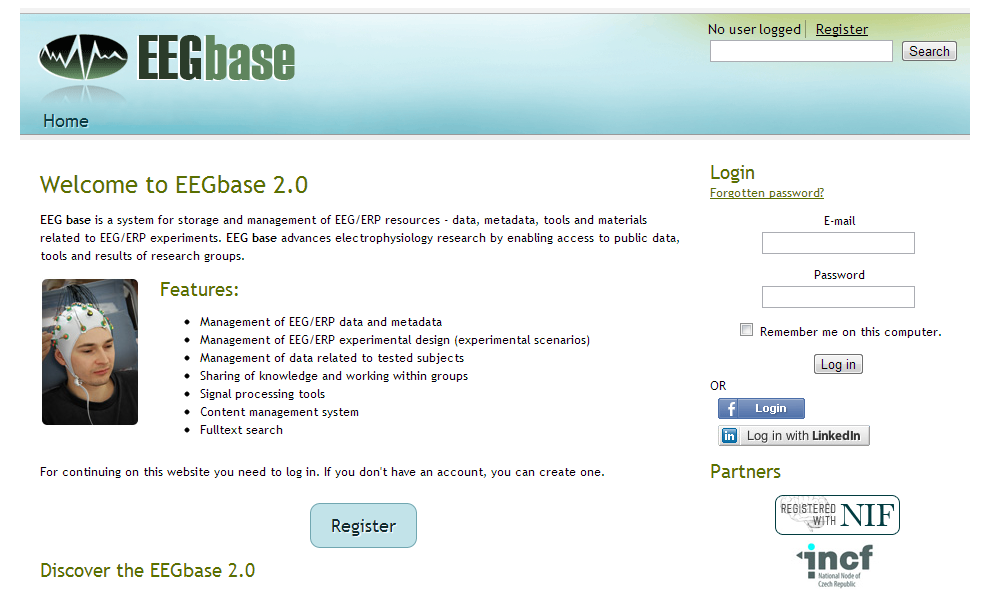
\includegraphics[width=1.00\textwidth]{figures/eegPortal.png}
	\caption{EEG/ERP Portal Welcome Page.}
	\label{fig:eegPortal}
\end{figure}


\subsubsection*{Hibernate}

% Strucne popsat, k cemu je Hibernate a jaky vyuziti ma v portalu. Mozna taky vlozit nejaky schema (z BP?)
Hibernate \cite{Hibernate:Home} is an open-source object-relational mapping framework, whose purpose is to facilitate storage and retrieval of Java domain objects. It is used in EEG/ERP Portal to map its domain model to ...

\subsubsection*{Spring Framework}

% Popsat strucne, jak funguje, jak se vyuziva
The Spring Framework facilitates creating Java-based enterprise applications. It applies a principle called dependency injection which helps to make the classes loosely coupled. The idea of this principle is to let the framework do all necessary wiring of objects, so that the objects can focus on their core responsibilities. 

\subsubsection*{Wicket}

% Popsal v par vetach a uvest, proc se na nej preslo.
... The EEG/ERP Portal's presentation layer is being developed in Wicket by the time of writing this thesis. It is a replacement of JSP pages and Spring MVC. This decision was made due to clearer separation of application logic and markup.





\part{Practical Part}


\chapter{Analysis}


\section{Choice of full text search solution}

From the search engines listed in previous parts of the thesis and technologies on which EEG/ERP Portal is based, the choice of the search engine can be restricted by the following criteria:

Speed - Based on the comparison made in chapter 3, the most performant search engines are ... and Lucene and all those built on Lucene

integration with EEG/ERP Portal - EEG/ERP Portal is based on Java technologies and this is why search engines providing Java API are easier to be integrated to the working infrastructure.

Other features and extensions - Because full text search
engines as they are take care of indexing and searching data, it is desirable to have a set of ``helper tools'' (such as result highlighting, faceted search, synonym search and more-like-this search) to make building full text search easier. It is considered natural for the end user to use the fulltext search with some of such tools implemented. 

Independence on data sources - The chosen search engine must be able to accept data from various sources and not be limited to only one specific data source, such as relational database. The reason behind this is the mentioned need to index LinkedIn articles as well as to enable possible furter indexing scenarios in the future, such as indexing .pdf or XML files.

Independence on other technologies - This criterion means that the search engine should not rely on a specific technology to be used. Dependence of Hibernate Search on Hibernate or ... on MySQL may serve as examples of the search engines which perform well is the conditions are met, but cannot work if not. 

Community - Numerous and active developer community also plays a big role in the final choice. The bigger community around the search engine is, the higher is the chance that the engine development will not stop early, new features will be introduced and that found bugs will be resolved quickly. Although one-man projects can look very promising and their future development is more likely to be managed by still growing community, 
A well documented project, many available tutorials and active user groups are a good sign of project stability and ensure that there will be someone ready to help to solve problems.

TODO MODIFY the table.

\begin{tabular}{|c|c c c c c|}
\hline

\textbf{Search Engine } & \textbf{Speed} & \textbf{Integration} & \textbf{Extension} & \textbf{Independence} & \textbf{Community} \\
\hline
Indri & Excellent & OK & KO & OK & 1 \\
\hline
Sphinx & Excellent & OK & KO & OK & 3 \\
\hline
Lucene & Excellent & OK & OK & OK & 5 \\
\hline
Zettair & Excellent & KO & KO & OK & 1 \\
\hline
Xapian & Good & OK & OK & OK & 1 \\ 

\hline
\end{tabular}
	
\section{How Lucene works}


\section{Instalation}

Distributed as a .war archive

HttpSolrServer and EmbeddedSolrServer


%\section{Solr and NoSQL}


\section{Solr Index}

Todo


\section{Ways of Indexing in Solr}

Todo

DataImportHandler vs. SolrJ

DataImportHandler (DIH) offers fast indexing of data from relational databases. The extraction of data to be added to the index as documents is based on creating custom SQL results. 
The drawback of DIH is its inflexibility. After each change of the relational schema the SQL queries which fetch the indexing data must be changed accordingly. Also the logic in the form of the SQL queries is out of reach of the EEG/ERP Portal application logic since the queries must be written in a special configuration file managed by the Solr server.

Disadvantages:

\begin{itemize}

\item Data model changes - For indexing of new data and enabling delta imports, it is necessary to add a new column to each table we wish to index. The column contains a timestamp for each record, holding the value of time of the last indexing.

\item After deletion of data in the database, certain actions must be taken to enable DIH to reflect these changes in the index. 
One way to do this is to browse the documents in the index and compare their ids with ids of their matching database records. If a document has no equvalent database record, it means that the record was deleted. After the comparison, redundant documents in the index are identified. This approax does not perform well.
Another way is to add an extra column that captures deletion times. Deletion times together with the record identification are added before the physical deletion of records. DIH can then get all records from the last executed crawl. An appropriate function and before delete trigger must be created for this solution. 

\item if the database schema changes - affected SQL queries must be rewritten to make them work again. SOLR schema changes is related to this matter as well. 

\end{itemize}

SolrJ - possibilities:
\begin{itemize}
\item @Field annotation SolrJ API in combination with addBean()/addBeans() methods.
The usage of provided annotations brings a problem of ambiguity of mapped objects. Documents stored in the Solr index must posess an identifier which is unique across all stored documents. Object ids are unique only in the class scope, so global uniqueness is not ensured. (pouziti Solr UUID nebylo
prostreleno). It is true that this way of making input documents is clear and easy. Unfortunatelly, its usage for more advanced scenarios is limited. This limitation lies in the unability to use the @Field annotation for fields which are Java objects and collections. Annotating just primitive or String value fields does not offer 

\item aspects - they are suitable for injecting cross-cutting concerns such as logging and database transactions to avoid spreading the same lines of code across the whole application. 
In our case, the existing need for indexing domain objects can be realized by simply enriching the base DAO methods responsible for creating, updating and deleting an object. This way the indexing calls happen only in a few known places in code. Introducing an extra aspect for this situation is more likely to be overkill, not to mention added complexity in debugging.

\item Integration with Hibernate Search and using its annotation mechanisms
The core idea of this proposed alternative is to use Hibernate Search for the initial phase of indexing, which includes creating input documents for indexing which happens automatically. The created documents would be handed over to Solr.
But - there would be an extra dependency on another technology. Besides, to cover indexing of data not present in the database another indexing mechanisms for these kinds of data would have to be created anyway. 

\item Custom annotation mechanism. By using the possibilities offered by Java Reflection, one cannot be limited by offered solutions and create a new one that overcomes found problems. There are some challenges, but it gives more freedom than previously proposed solutions. It would be desirable to create a solution universal for all domain objects. Inspired by the provided SolrJ annotations. It also involves creating a custom code to implement generating a unique id for each created document.  Bylo by vyuzito reflexe a zajistena

\item filter - web.xml
\end{itemize}

\section{Integration}

Todo


\section{SolrJ}

Solr provides a Java API for integration of Java applications with the Solr server called SolrJ API.


\chapter{Index design}

Je dulezite si pri navrhu indexu uvedomit, ze dokumenty
ulozene v indexu zachycuji informace, ktere jsou vyhledavany. Je proto
nutne znat poradne povahu a ucel fulltexoveho vyhledavani
v dane domene. Tento fakt je pro indexaci dokumentu zvlast
dulezity, protoze dokumenty ukladane v indexu maji jista specifika
a omezeni, ktere jsou rozebrany v nasledujicich odstavcich.


\section{Search Requirements}

The current version of EEG/ERP Portal uses Hibernate Search to implement
the fulltext search feature. This framework is sufficient for dealing
with input data coming only from a database data source. This is because
of the fact that the technology is based on Hibernate, a powerful
object-relational mapping framework. Hibernate Search uses internally
Lucene and Solr analyzers to provide the full text search itself.
However, the current implementation suffers from several issues which
are desired to be fixed. The highlighting functionality does not work
as expected in certain cases. 


\section{Index Structure Specifics}

Compared to traditional relational databases, the Solr index lacks
the possibility to create more structured content. An analogy to the
index would be a single large table in the relational world. As a
relational table, index structure is flat and does not allow nesting
documents to form hierarchical structures as in the case of document
databases like MongoDB.

...Index ma plochou strukturu, neumoznuuje vnorovat dokumenty
do sebe, jako v pripade dokumentovych databazi. lze vsak imitovat
relaci 1:N pomoci multivalued fields, ktere jsou ulozeny ve forme
pole.

Reprezentaci dokumentu lze vyresit nekolika zpusoby:
\begin{itemize}
\item Denormalizace relacnich dat
\item Od Solr 4 podpora join funkce. Dost omezene oproti SQL joinu
\item nekolik po sobe nasledujicich dotazu, nasledujici dotaz
bere jako vstup vysledky predchoziho dotazu.
\end{itemize}

\subsection{Eventual consistency}

za pouziti real-time indexovani. po insertu, updatu, deletu dochazi
k indexaci prislusneho dokumentu.

Sekvence insert/update/delete a indexace neprobiha atomicky jako transakce.
Pri chybe muze dojit k nekonzistentnimu stavu (data ulozena,
indexovana -> OK; data ulozena, ale neindexovana -> nebudou vyhledatelna;
data neulozena, indexovana -> nalezeny neodpovidajici nebo neexistujici
vysledky; data neulozena, neindexovana -> DB rollback, puvodni
zaznam lze vyhledat . Osetreni konzistence v techto pripadech
byva netrivialni zalezitost, casto realne resitelna jen
castecne. Beznym resenim nekonzistentnich stavu
je je ignorovat, protoze nakonec budou po dalsi naplnnovani reindexaci
odstraneny. Tim je dosazeno. tzv. eventual consistency.


\chapter{Fulltext Search Design}

Previous parts of the thesis shown that documents in index and records
stored in relational database tables serve to different purposes and
use cases und therefore must be treated differently. The treatment
in this context means storing, structuring and saving the data.

Being aware of the index structure and its specifics, it is almost
always necessary to make a kind of transformation from the relational
to the index form in order to make the full text search work properly
and efficiently. There are several ways to accomplish this goal, one
of them involves flattening the relational structure. This leads to
denormalized data which is mostly unacceptable in relational databases,
but since index is quite different from databases, denormalization
is even desired. The main thing one should know when desiging an index
structure is to know which search results a user expects and how the
final representation of full text results should look like.

Pokud bychom zvolili pristup of direct 1:1 mapping of entities to the indexu,
dostaneme pro kazdou entitu odpovidajici typ dokumentu, ktery obsahuje
zvolene indexovane polozky pro danou entitu. 


\chapter{Implementation}


\section{Java Reflection}

Reflection is the ability to inspect the code and make its modifications at runtime. It is a feature that makes languages like Java more dynamic. Its heavy usage can be found especially in modern frameworks such as Spring or Hibernate, that both use reflection for instatiating classes from information in configuration files. 

A very common use case of reflection in Java is the usage with annotations. This combination opens many possibilities of manipulating class metadata. In JUnit 4, for example, the @Test annotation was introduced. The JUnit framework looks up all methods marked by this marker annotation and call them in each execution of running unit tests.

The root class of the Java object hierarchy, the Object class, has the method getClass() providing the corresponding Class object, meaning that all Java classes can be invoked or inspected by means of reflection.

%Co to je, na co se pouziva, jak se pouziva v implementaci
%
%The name reflection is used to describe code which is able to inspect other code in the same system (or itself).
%
%One very common use case in Java is the usage with annotations. JUnit 4, for example, will use reflection to look through your classes for methods tagged with the @Test annotation, and will then call them when running the unit test.
%
 %The ability to inspect the code in the system and see object types is Type Introspection. Reflection is then the ability to make modifications at runtime by making use of introspection.
%
 %For example, all objects in Java has the method getClass, which lets you determine its class even if you don't know it at compile time (like if you declared it as Object) - this might seem trivial, but such reflection is not by default possible in less dynamic languages such as C++.
%
%Take for example your typical web.xml file. This will contain a list of servlet elements, which contain nested servlet-class elements. The servlet container will process the web.xml file, and create new a new instance of each servlet class through reflection.
%
%Reflection is important since it lets you write programs that does not have to "know" everything at compile time, making them more dynamic, since they can be tied together at runtime. The code can be written against known interfaces, but the actual classes to be used can be instantiated using reflection from configuration files.
%
%Lots of modern frameworks uses reflection extensively for this very reason. the most comprehensive example is Spring which uses reflection to create its beans, and for its heavy use of proxies
%
%It's useful in a lot of situations. Everywhere you want to be able to dynamically plug in classes into your code. Lot's of object relational mappers use reflection to be able to instantiate objects from databases without knowing in advance what objects they're going to use. Plug-in architectures is another place where reflection is useful. Being able to dynamically load code and determine if there are types there that implement the right interface to use as a plugin is important in those situations.

\section{REST}

REpresentational State Transfer
co to je


\section{LinkedIn API}

LinkedIn provides REST API to access to various information. Required information one wishes to obtain can be specified by URI parameters in the JSON format. 
co vratit, jestli posts, users, groups
etc. a jak detailne (jestli napr. u posts vratit i popis,
timestamp, id,...). Spring poskytuje metody, ktere obaluji REST volani,
nekdy ale neposkytuji, co je zrovna potreba (treba nevraci
timestamp a summary u articles). Lze ovsem vytvorit
vlastni REST volani a nechat si vratit data, ktera zrovna potrebujeme.

Indexers

An annotation interface was created to cover indexing data. 
Pro efektivni
searching bylo potreba indexovat dokumenty, ktere represent
denormalizoed data. Bylo nutne rozlisit rodicovske objekty a
podrazene objekty, ktere rodicovske objekty obsahuji jako
property nebo ve svych kolekcich. Prikladem muze byt rodicovsky
objekt experiment, ktery obsahuje kolekci podrazenych hardware
objektu.


\section{Hibernate lazy vs. eager loading}

explain pojem dynamic proxy pattern, ktery Hibernate pro eager
loading pouziva.

A program may consist of several domain objects which contain a reference
to another domain object or to a collection of objects. Most of the
time when accessing a certain domain object it is enough to get only
the fields of primitive types and associated collections are not needed.
This prevents Hibernate from performing additional unnecessary queries.

U lazy loadingu jde o usporu nepotrebnych dotazu, tim padem
mensi rezii a tim urychleni behu aplikace. Lazy loading je proto
uprednostnovan a pro kolekce, tedy vazby 1:N, je v Hibernate
nastaven jako default. Pokud vsak potrebujeme pristoupit
k objektum v kolekci lazily loaded objektu, dostaneme LazyInitializationException,
protoze objekty nebyly do kolekce nacteny.

Naproti tomu eager loading pri prvnim pristupu k objektu vytvori
instance pro vsechny objekty, na ktere ma ziskany objekt vazbu. Tento
approach je pametove narocnejsi, zpomaluje
beh aplikace a mel by se pouzit jen v pripadech, kdy jsme
si jisti, ze budeme potrebovat informace o associated objects.

V aplikaci portalu je z techto rozumnych reasons snaha pouzit lazy
loading, kde to jen jde. V common situations neni eager loading
zapotrebi, a proto... 

Pro indexaci dat je zapotrebi fetch data z databaze vcetne
vsech objektu, ktere k nim belong, aby se do indexu zachytily
informace i z techto podrazenych objektu.

Ensuring eager loading

- zmenou konfigurace Hibernate mapping. Neni pro nas suitable pristup,
protoze je malo flexible. Znamenalo by to, ze by se k vsem objects
nacitaly vsechny objekty s 1:N relaci. Dotazy by trvaly delsi
dobu, bylo by treba vice pameti, takze melo by to za nasledek
pomalejsi beh apliakce.

- custom HQL dotazy s fetchmode=``eager``. Je nutne psat zvlast
pro kazdou entitu dotaz, ve kterem uvedeme, ktere objekty chceme eager
fetchnout

- vyuziti metody Hibernate.initialize(), ktere se jako parametr preda
objekt, ktery ma byt k parent objektu pripojen. V kombinaci
s Java reflexi lze docilit univerzalniho solution pro vsechny objekty


\section{Indexing algorithm}


\section{Solr configuration}

\subsection{Handling synonyms}


\section{Periodic indexing}

Since LinkedIn articles can be added directly via LinkedIn from a user account and not via the form on the EEG/ERP Portal website, the portal application pri adding
articles takovymto zpusobem se o novych acticles nemuze
dozvedet. Proto u LinkedIn articles je potreba krome
indexovani i clanku pridanych z portalu zajistit i indexaci
clanku pridanych vne portal. Resenim je provadet
pravidelnou indexaci vsech clanku na LinkedInu. Objektova
reprezentace articles lze obdrzet pres LinkedIn API a ty
potom v pozadovane podobe predat indexeru. Zajisti se tim
pritomnost vsech publikovanych articles na LinkedInu v indexu.
Nevyhodou je fakt, ze nektere clanky budou indexovany se zpozdenim
danem v nejhorsim pripade periodou jejich indexovani. 

The Spring Framework has a native support of task scheduling and asynchronous
calls. Since its version 3.0, methods can be scheduled and also run
asynchronously by using annotations, namely the @Scheduled and @Async
annotations. The first mentioned annotation, when added to a method,
makes the method schedulable by Spring. Usage of this annotation is
restricted to the void methods with no parameters. The @Scheduled
annotation has to contain a piece of metadata to tell Spring how to
plan the method scheduling. Currently there are three available attributes
for the @Scheduled annotation, from which the most flexible option
is specifying a cron expression to trigger a task as shown on the
following lines:

\begin{verbatim}
@Scheduled(cron=* 0 22 * * SAT-SUN)
public void indexAll()
\end{verbatim}


This way, the method indexAll() will be scheduled to run every at
10 pm only on Saturday and Sunday. Cron syntax allows a user to create
more sophisticated scheduling scenarios, but discussing the syntax
is out of scope of this work. Since Spring is using Quartz as a scheduler
under the covers, an interested reader can find all necessary information
about the syntax in the Quartz documentation \cite{QuartzDoc}.


The @Async annotation is used to mark the methods to be invoked asynchronously.
It is very easy to use for methods having void return values:

\begin{verbatim}
@Async
public void indexLinkedIn()
\end{verbatim}


In order to enable annotation-based scheduling it is necessary to
add a new element in the application context file as well as the task
namespace to which the element belongs.

\begin{verbatim}
<xmlns:task="... http://www.springframework.org/schema/task" 
xsi:schemaLocation="... http://www.springframework.org/schema/task/spring-task.xsd">
...
<task:annotation-driven executor="indexingExecutor" scheduler="indexingScheduler"/>
\end{verbatim}


The annotation-driven element requires executer and scheduler attributes
to be set to handle tasks represented by methods marked by @Async
and @Scheduled annotations, respectively.

\begin{verbatim}
<task:executor id="indexingExecutor" pool-size="5"/> 
<task:scheduler id="indexingScheduler" pool-size="1"/>
\end{verbatim}




,,Notice that an executor reference is provided for handling those
tasks that correspond to methods with the @Async annotation, and the
scheduler reference is provided for managing those methods annotated
with @Scheduled.``


\section{User Interface}

\subsection{Search Form}

\subsubsection{Autocomplete}

\subsection{Search Results}

\chapter{Testing}
\label{chap:testing}

% http://vrtoonjava.wordpress.com/2012/06/17/part-3-dao-and-service-layer/ - testing section

This chapter presents created test cases to prove the correct functionality of the implementation of the full text search for the EEG/ERP Portal. The tests are of two types. The first type of the tests are JUnit tests which cover the functionality on the core, application logic level. The second test category includes Selenium tests whose purpose is to simulate user interaction with the full text search.

All tests use the test data from the database server and interact with an independently running Solr test server to access indexed data. The server runs at the address 147.228.63.134 on port 8686 (147.228.63.134:8686/solr/).

Although the tests could have been performed in combination with the embedded version of the Solr server, its remotely running instance imitates the production environment in a better way.

%Jako reseni se pro testovani nabizela take tzv. embedded verze Solr serveru (trida EmbeddedSolrServer).
%Protoze je server spojen s aplikaci, HTTP pristup je v tomto pripade
%jen simulovan, navic neumoznuje takove moznosti spravy a nastaveni
%jako samostatne bezici server. Proto byla dana prednost
%samostatne instanci Solru, ktera verohodneji imituje provoz
%na ostrem Solr serveru.


\section{Unit Tests}

There were several test cases created by using JUnit4. It was possible to integrate JUnit with Spring in order to use declared Spring beans in the test cases. 
Their main purpose is to verify expected functionality of various classes related to the full text search.

\subsection{FulltextSearchServiceTest.java}

This test class uses the \texttt{FulltextSearchService} class to test its autocomplete and faceting functionality.
The \texttt{getAutocompleteResultsSuccess()} and \texttt{getAuto\-complete\-Results\-Fail()} tests the autocomplete part.
As their names say, these methods test returning the expected output for two different input strings. 
In case of the first mentioned test, the test passes if any autocomplete suggestions are found for the query string.
On the contrary, the other test passes if a given search string outputs no autocomplete results.

Faceted search is covered by the \texttt{get\-Document\-Count\-For\-Empty\-Query()}, \texttt{facet\-All\-Test()} and \texttt{facet\-None\-Test()} tests.
\texttt{getDocumentCountForEmptyQuery()} tests obtaining the zero number of search results if an empty string is searched.
The \texttt{facet\-All\-Test()} and \texttt{facet\-None\-Test()} methods test creating faceted categories.
The \texttt{facetAllTest()} test passes if the number of documents in each category is greater than zero if all documents are retrieved (by using the * sign as the input query). 
\texttt{facetNoneTest()} uses the empty search string that should not return any documents. Therefore, this test succeeds if the number of documents in each category is equal to zero.

\subsection{IndexingServiceTest.java}

This class contains tests of methods of the \texttt{IndexingService} class.

\subsection{IndexingTest.java}

It contains methods that test indexing created sample documents and their removal from the Solr index.
For example, the \texttt{indexSampleIndexablePojos()} method is a test case that creates an instance of each indexable parent class and performs a query that returns all documents representing these instances. This test succeeds if all created documents are returned by the query.

\subsection{LinkedInIndexingTest.java}

This test class contains JUnit tests that check the correct behavior of manipulation with received LinkedIn articles via the LinkedIn REST API.

\section{Integration Tests (Selenium)}

These tests were created to simulate actions of users using the full text search of EEG/ERP Portal. 
The tests deal with:

% Popis testu
\begin{itemize}
	\item checking the presence of web elements, such as the search panel and the search button in the main menu
	\item testing the autocomplete box
	\item testing obtaining any search results for a given search query
	\item checking that, for a search query returning no results, a corresponding message appears and no results are shown.
\end{itemize}

% TODO nefungujou Selenium testy



\chapter{Conclusion}

% *************** Bibliography ***************
\bibliographystyle{ieeetr}
\bibliography{bibliography}

%\printbibliography
%\begin{thebibliography}{}
%\end{thebibliography}

\end{document}
